\lab{Solitons}{Solitons}
\label{lab:solitons}

\objective{
We study traveling wave solutions of the Korteweg-de Vries (KdV) equation, using a pseudospectral discretization in space and a Runge-Kutta integration scheme in time.  }

Here we consider soliton solutions of the Korteweg-de Vries (KdV) equation. This equation is given by 
\[  \frac{\partial u }{\partial t} + u \frac{\partial u}{\partial x} + \frac{\partial^3 u}{\partial x^3} = 0.
\]
The KdV equation is a canonical equation that describes shallow water waves. 

The KdV equation possesses traveling wave solutions called solitons.  
These traveling waves have the form 
\[ u(x,t) = 3s \sech^2\left(\frac{\sqrt{s}}{2}(x - st - a)\right),
\]
where $s$ is the speed of the wave. 
Solitons were first studied by John Scott Russell in 1834, in the Union Canal in Scotland. 
When a canal boat suddenly stopped, the water piled up in front of the boat continued moving down the canal in the shape of a pulse.  

Note that there is a soliton solution for each wave speed $s$, and that the amplitude of the soliton depends on the speed of the wave. 
Solitons are traveling waves in the shape of a pulse, they are nonlinearly stable (bumped waves return to their previous shape), and they maintain their energy as they travel. 
They also enjoy an additional stability property: they play well with others. 
Two interacting solitons will maintain their shape after crossing paths. 

\section*{Numerical solution}
Consider the KdV equation on $[-\pi,\pi]$, together with an appropriate initial condition: 
\begin{align*}
	 &{ }u_t = -\left(\frac{u^2}{2} \right)_x - u_{xxx},\\
     &{ }u(x,0) = u_0(x).
\end{align*}
We will use initial data that is zero at the endpoints.
This will allow us to use a pseudospectral method for periodic initial data to find a numerical approximation for the solution $u(x,t)$. 

If we use $N$ subintervals in space, we then obtain the spatial step $h = 2\pi/N$ and the grid points $\{x_j\}_{j=1} = \{-\pi,-\pi + h,\ldots,\pi-h\}$.  
Let $\mathcal{F}(u)(t) = \hat{u}(t)$ denote the Fourier transform of $u(x,t)$ (in space), so that 
\[
\mathcal{F}(u) = \hat{u}(k,t), \quad k=-N/2+1, \ldots, N/2.
\]
Similarly we let $\mathcal{F}^{-1}$ represent the discrete inverse Fourier transform.
Recall that $k$ represents the wave numbers in Fourier space; our code defines it by 
\begin{lstlisting}
# Array of wave numbers.  This array is reordered in Python to 
# accomodate the ordering inside the fft function in scipy.
k = np.concatenate(( np.arange(0,N/2) ,
					 np.array([0])	,
					 np.arange(-N/2+1,0,1)	)).reshape(N,)
\end{lstlisting}

We now apply the Fourier transform to the KdV equation.
In Fourier space, we obtain 
\begin{align*}
	\mathcal{F}(u)_t &= -\frac{ik}{2}\mathcal{F}(u^2)- (ik)^3\mathcal{F}(u).
\end{align*}
Let $U(t)$ be the vector valued function given by $U(t) = (u(x_j,t))_{j=1}^N$.
Let $\mathcal{F}(U)(t)$ denote the discrete Fourier transform of $u(x,t)$ (in space), so that 
\[
\mathcal{F}(U)(t) = (\mathcal{F}(u)(k,t))_{k=-N/2+1}^{N/2}.
\]
Similarly we let $\mathcal{F}^{-1}$ represent the discrete inverse Fourier transform.
Using the pseudospectral approximation in space leads to the system of ODEs
\begin{align}
	\mathcal{F}(U)_t =  -\frac{i}{2} \vec{k}\mathcal{F}\left( \mathcal{F}^{-1}(\mathcal{F}(U))^2\right) + i\vec{k}^3\mathcal{F}(U)
\end{align}
where $\vec{k}$ is a vector, and multiplication is done element-wise. In terms of $Y = \mathcal{F}(U)$, this simplifies to 
\begin{align}
	Y_t =  -\frac{i}{2} \vec{k}\mathcal{F}\left( \mathcal{F}^{-1}(Y)^2\right) + i\vec{k}^3Y
	\label{lab:solitons:pseudospectral}
\end{align}
and is implemented below.
\begin{lstlisting}
# Defines the left hand side of the ODE y' = G(t,y)
# defined above.
ik3 = 1j*k**3.
def G_unscaled(t,y):
	out = -.5*1j*k*fft(ifft(y,axis=0)**2.,axis=0)  + ik3*y        
	return out
\end{lstlisting}

Equation \eqref{lab:solitons:pseudospectral} is solved below, using a soliton as initial data for the KdV equation. 
Note that the Fourier transform must be applied to the soliton before solving, and that the final numerical solution must be transformed back from Fourier space before plotting. 
\begin{lstlisting}
N = 256
x = (2.*np.pi/N)*np.arange(-N/2,N/2).reshape(N,1)   # Space discretization
s, shift = 25.**2., 2.  							# Initial data is a soliton
y0 = (3.*s*np.cosh(.5*(sqrt(s)*(x+shift)))**(-2.)).reshape(N,) 

# Solves the ODE.
max_t = .0075
dt = .2*N**(-2.)
max_tsteps = int(round(max_t/dt))
y0 = fft(y0,axis=0)
T,Y = RK4(G_unscaled, y0, t0=0, t1=max_t, n=max_tsteps)

# Using the variable stride, we step through the data, 
# applying the inverse fourier transform to obtain u.
# These values will be plotted.
stride = int(np.floor((max_t/25.)/dt))
uvalues, tvalues = np.real(ifft(y0,axis=0)).reshape(N,1), np.array(0.).reshape(1,1)
for n in range(1,max_tsteps+1):
	if np.mod(n,stride) == 0:
		t = n*dt
		u = np.real( ifft(Y[n], axis=0) ).reshape(N,1)
		uvalues = np.concatenate((uvalues,np.nan_to_num(u)),axis=1)
		tvalues = np.concatenate((tvalues,np.array(t).reshape(1,1)),axis=1)

fig = plt.figure()
ax = fig.gca(projection='3d')
ax.view_init(elev=45., azim=150)
tv, xv = np.meshgrid(tvalues,x,indexing='ij')
surf = ax.plot_surface(tv,xv, uvalues.T, rstride=1, cstride=1, cmap=cm.coolwarm,
						linewidth=0, antialiased=False)
tvalues = tvalues[0]; ax.set_xlim(tvalues[0], tvalues[-1])
ax.set_ylim(-pi, pi); ax.invert_yaxis()
ax.set_zlim(0., 4000.)
ax.set_xlabel('T'); ax.set_ylabel('X'); ax.set_zlabel('Z')
plt.show()
\end{lstlisting}

The method we have used requires the use of an algorithm for (ODE) initial value problems, such as the RK4 algorithm.
The RK4 method is implemented below.
\begin{lstlisting}
def initialize_all(y0, t0, t1, n):
	""" An initialization routine for the different ODE solving
	methods in the lab. This initializes Y, T, and h. """
	
	if isinstance(y0, np.ndarray):
		Y = np.empty((n, y0.size),dtype=complex).squeeze()
	else:
		Y = np.empty(n,dtype=complex)
	Y[0] = y0
	T = np.linspace(t0, t1, n)
	h = float(t1 - t0) / (n - 1)
	return Y, T, h

def RK4(f, y0, t0, t1, n):
	""" Use the RK4 method to compute an approximate solution
	to the ODE y' = f(t, y) at n equispaced parameter values from t0 to t
	with initial conditions y(t0) = y0.
	
	'y0' is assumed to be either a constant or a one-dimensional numpy array.
	't0' and 't1' are assumed to be constants.
	'f' is assumed to accept two arguments.
	The first is a constant giving the current value of t.
	The second is a one-dimensional numpy array of the same size as y.
	
	This function returns an array Y of shape (n,) if
	y is a constant or an array of size 1.
	It returns an array of shape (n, y.size) otherwise.
	In either case, Y[i] is the approximate value of y at
	the i'th value of np.linspace(t0, t, n).
	"""
	Y, T, h = initialize_all(y0, t0, t1, n)
	for i in xrange(1, n):
		K1 = f(T[i-1], Y[i-1])
		tplus = (T[i] + T[i-1]) * .5
		K2 = f(tplus, Y[i-1] + .5 * h * K1)
		K3 = f(tplus, Y[i-1] + .5 * h * K2)
		K4 = f(T[i], Y[i-1] + h * K3)
		Y[i] = Y[i-1] + (h / 6.) * (K1 + 2 * K2 + 2 * K3 + K4)
	return T, Y
\end{lstlisting}

\begin{figure}
\centering
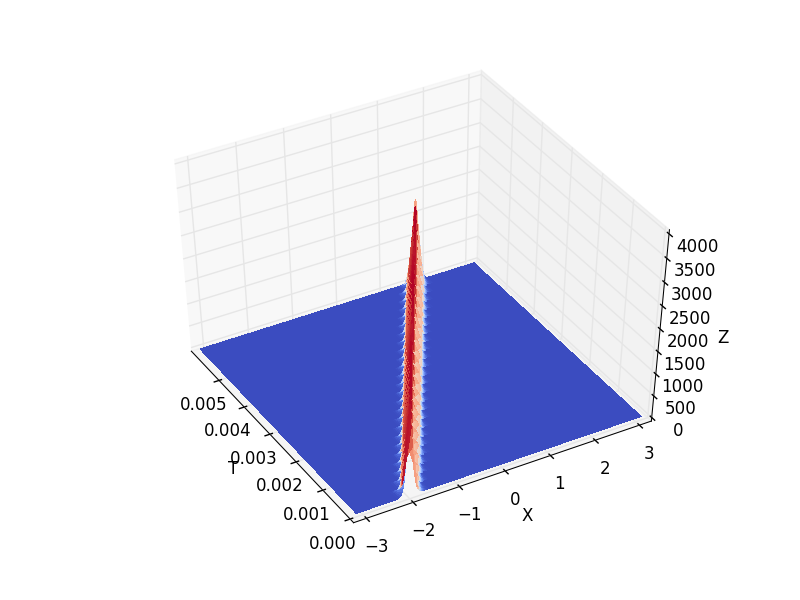
\includegraphics[width=\textwidth]{soliton.png}
\caption{The solution to Problem \ref{problem:solitons:single}.}
\label{fig:solitons:single}
\end{figure}

\begin{problem}
Run the code above to numerically solve the KdV equation on $[-\pi,\pi]$ with initial conditions 
\[
u(x,t=0) = 3s\sech^2\left(\frac{\sqrt{s}}{2}(x+a)\right),
\]
where $s = 25^2,$ $a = 2$. Solve on the time domain $[0,.0075]$.
The solution is shown in Figure \ref{fig:solitons:single}.
\label{problem:solitons:single}
\end{problem}

\begin{figure}
\centering
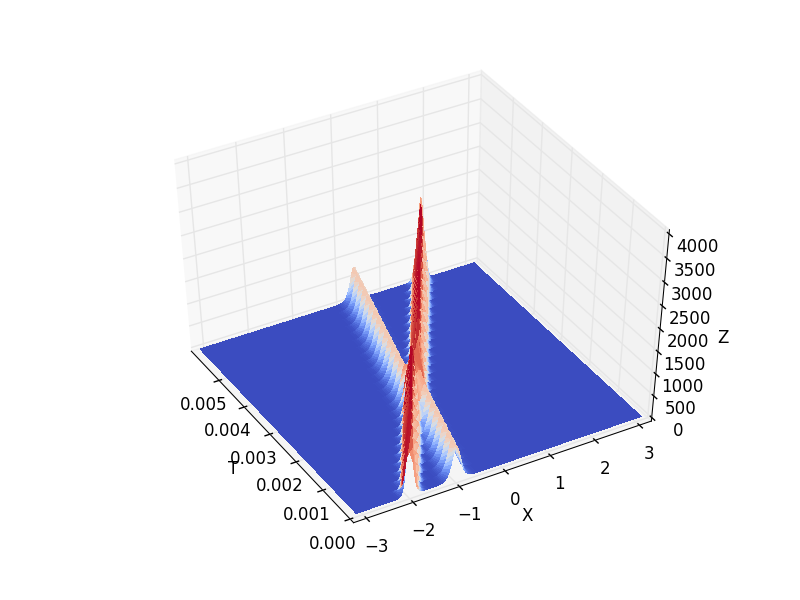
\includegraphics[width=\textwidth]{interacting_solitons.png}
\caption{The solution to Problem \ref{problem:solitons:interacting}.}
\label{fig:solitons:interacting}
\end{figure}

\begin{problem}
Numerically solve the KdV equation on $[-\pi,\pi]$.
This time we define the initial condition 
to be the superposition of two solitons,
\[
u(x,t=0) = 3s_1\sech^2\left(\frac{\sqrt{s_1}}{2}(x+a_1)\right) + 3s_2\sech^2\left(\frac{\sqrt{s_2}}{2}(x+a_2)\right),
\]
where $s_1 = 25^2,$ $a_1 = 2$, and $s_2 = 16^2,$ $a_1 = 1$.\footnote{This problem is solved in \textit{Spectral Methods in MATLAB}, by Trefethen.}
Solve on the time domain $[0,.0075]$.
The solution is shown in Figure \ref{fig:solitons:interacting}.
\label{problem:solitons:interacting}
\end{problem}

\begin{problem}
Consider again equation \eqref{lab:solitons:pseudospectral}.
The linear term in this equation is $i\vec{k}^3Y$.
This term contributes much of the exponential growth in the ODE, and responsible for how short the time step must be to ensure numerical stability.
Make the substitution $Z = e^{-ik^3t}Y$ and find a similar ODE for $Z$.
This essentially allows the exponential growth to be scaled out (it's solved for analytically).
Use the resulting equation to solve the previous problem.
\end{problem}